In a typical instance of the current state of the art algorithm, the
continued fraction expansion (CFE), the expansion depends upon the
last ten elements in the input signal history.{\bf CITATION} To make a
fair comparison between fractional derivative or integral algorithms,
it we examine the average Grunwald algorithm with ten bins of input
signal history, such that the history memory requirement is the
same. Figure~\ref{fig:bode10p05} contains a bode plot for a fractional
derivative of order $\alpha=0.5$ with ten history registers. Compared
to the CFE10, the average Grunwald with an exponential binning
structure (EXP10) has an approximately half a decade gain in
constant-phase bandwidth. {\bf OVERSAMPLING}

The performance of the average Grunwald algorithm improves
dramatically with a small increase in the number of input signal
history bins. The number of input signal history bins was limited by
the computational abilities of the computer for both the CFE and the
average Grunwald algorithms. For the CFE, the maximum input signal
history depth was $40$ steps into the past. For the average Grunwald,
it was possible to run up to $26$ bins ($>10^7$ steps into the past
for exponential binning). Figure~\ref{fig:bode40_26} compares the $40$
history memory registers of the CFE to the $26$ history memory
registers of the average Grunwald, for a variety of binning
strategies. At low frequencies, we see that for both fractional
derivatives and integrals there is a gain in the constant phase
bandwidth of about a decade.

\begin{figure}
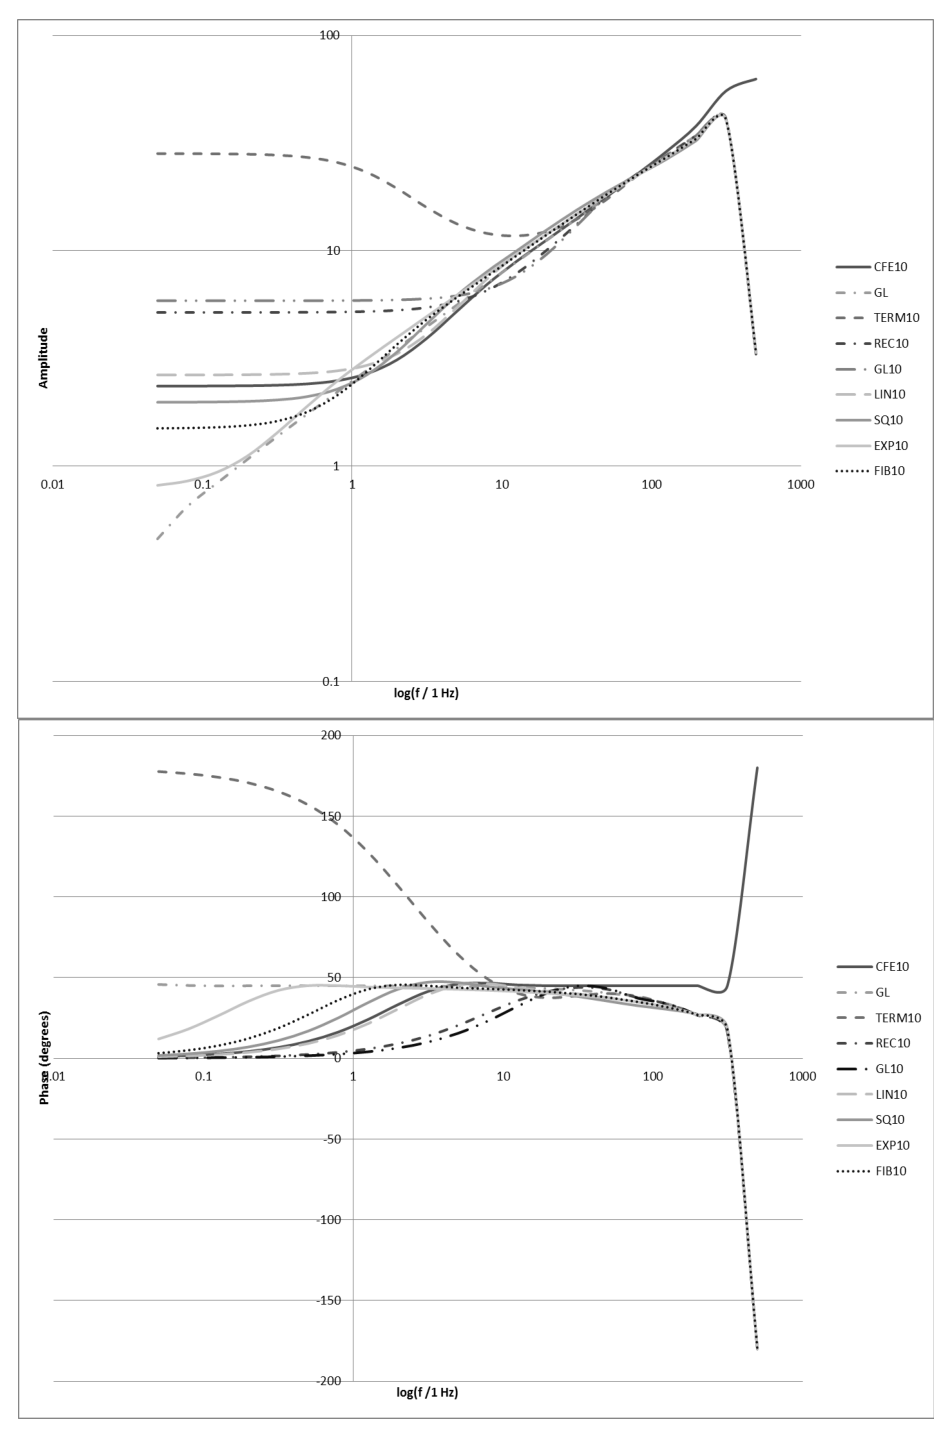
\includegraphics[width=2.5in]{bode10000_10_10_p05.eps}
\label{fig:bode10p05}
\caption{Amplitude and phase as a function of frequency for 10
  registers of binned (SQ10, EXP10, FIB10) or unbinned (GL10, CFE10)
  input signal history. GL is the full Grunwald calculation, for the
  entire input signal history prior to that time.}
\end{figure}

\begin{figure}[ht!]
\begin{center}
\subfigure{
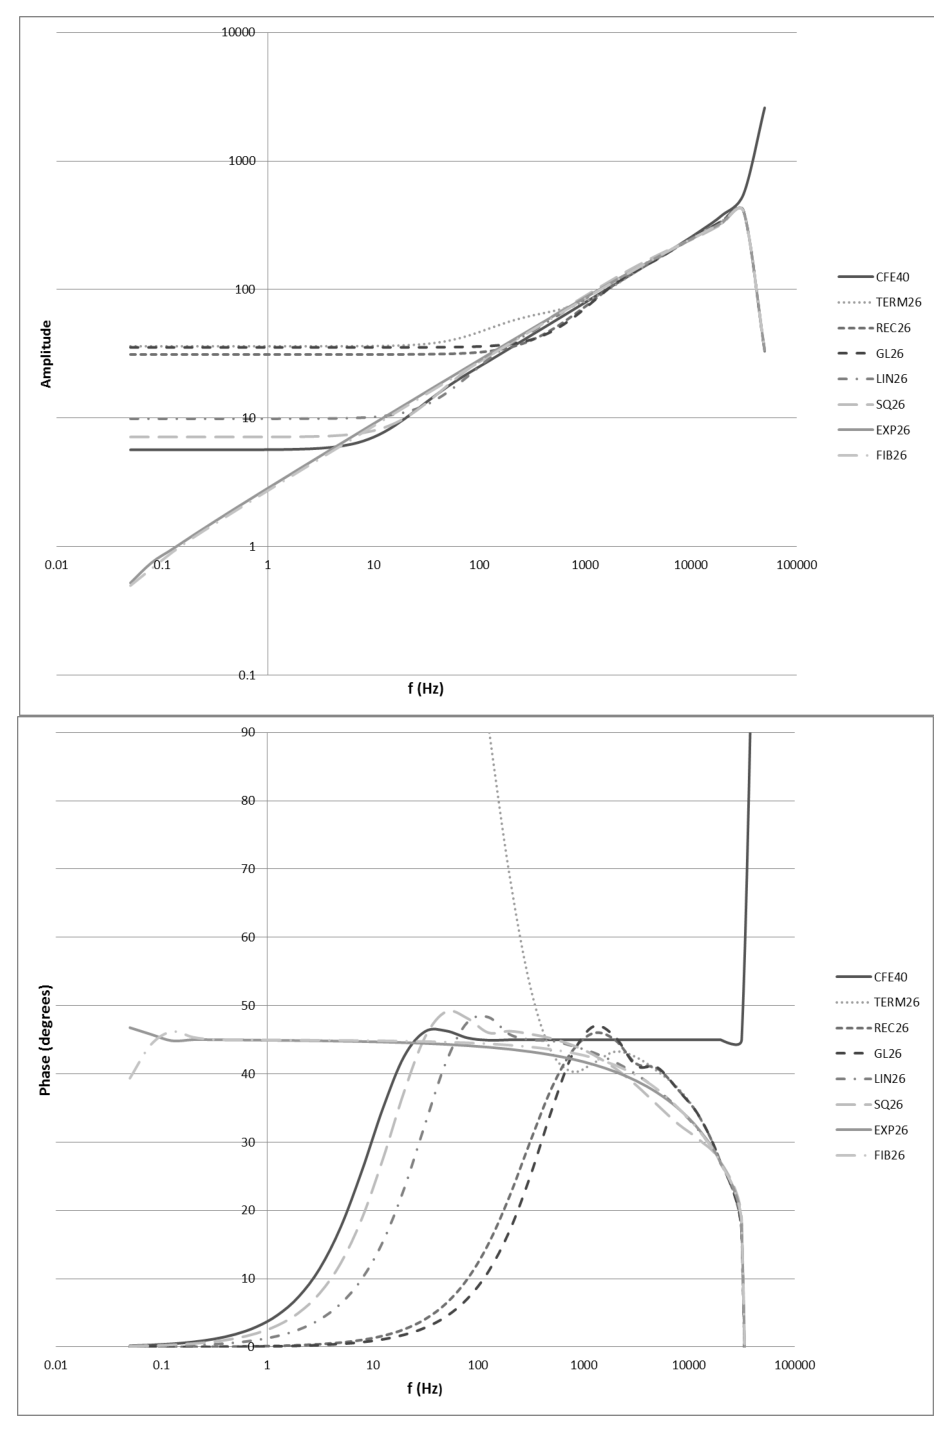
\includegraphics[width=2.5in]{bode1G_40_26_p05.eps}
}
\subfigure{
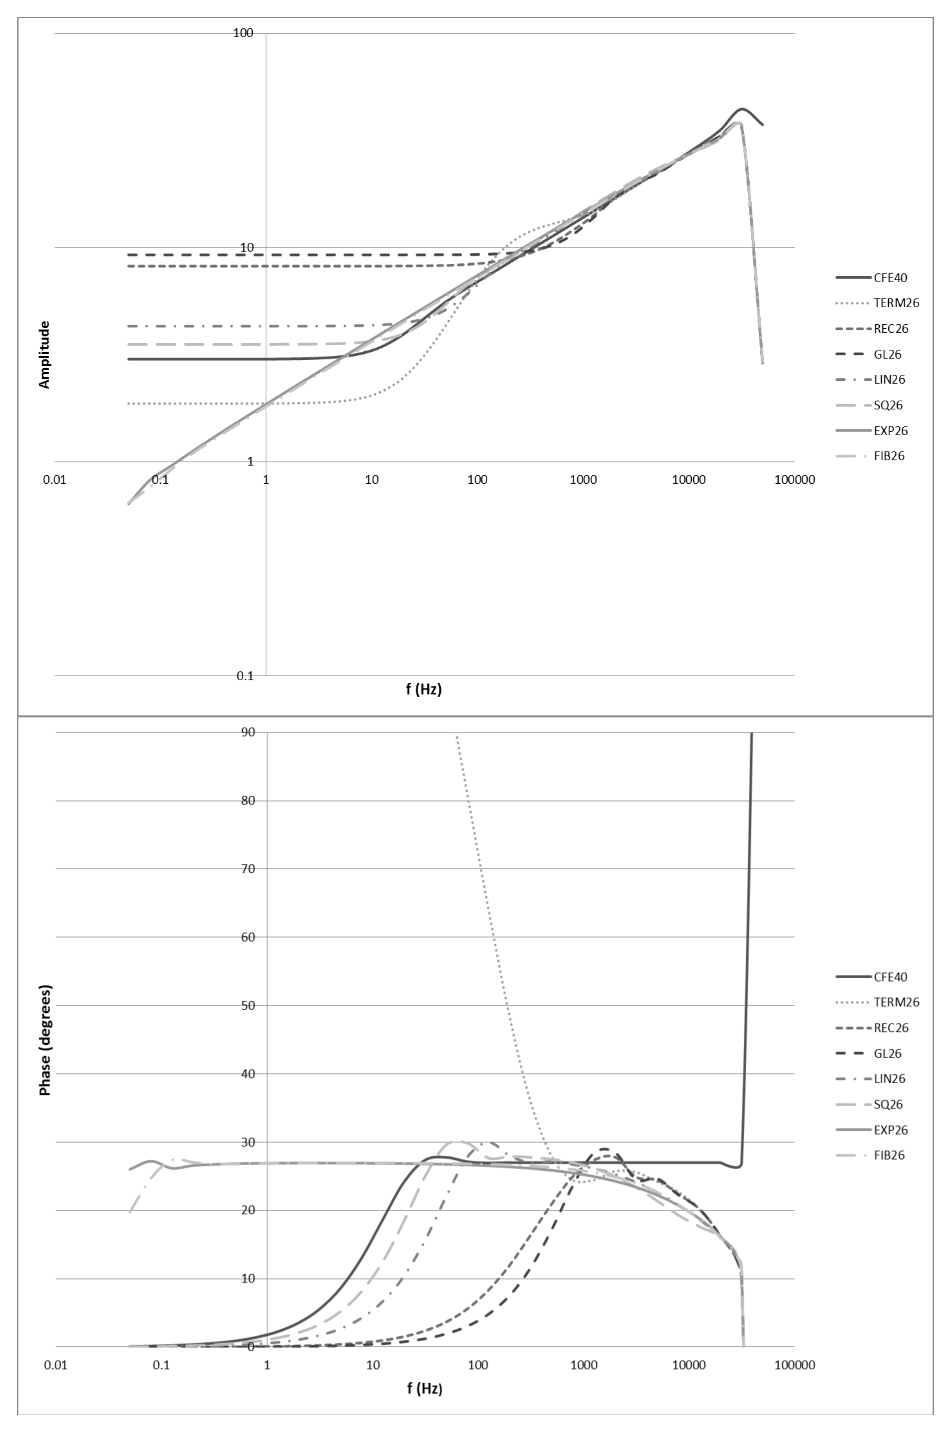
\includegraphics[width=2.5in]{bode1G_40_26_p03.eps}
}\\
\subfigure{
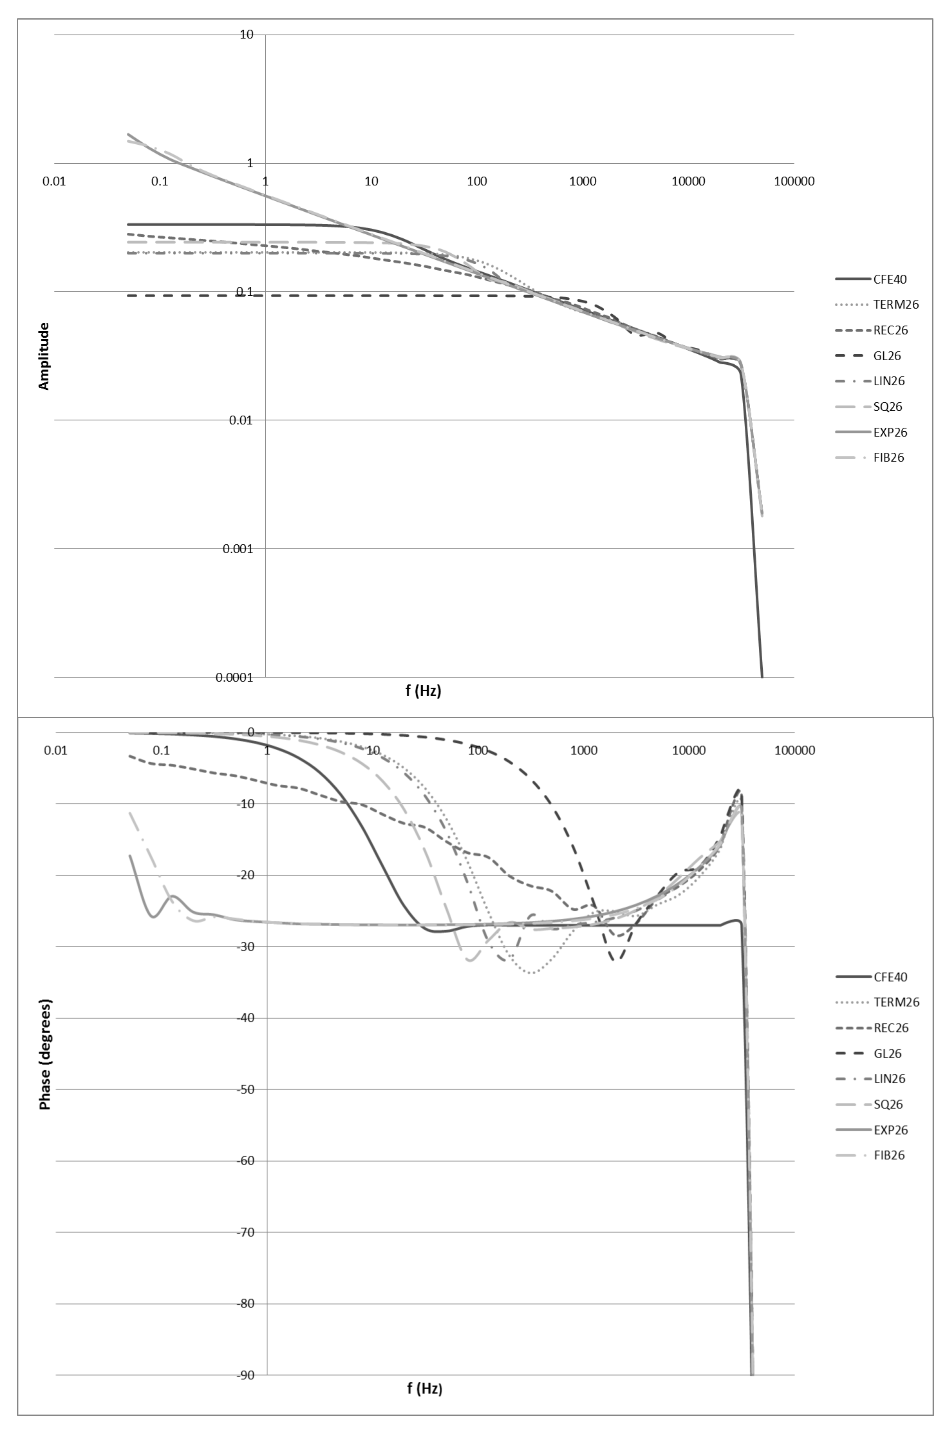
\includegraphics[width=2.5in]{bode1G_40_26_m03.eps}
}
\subfigure{
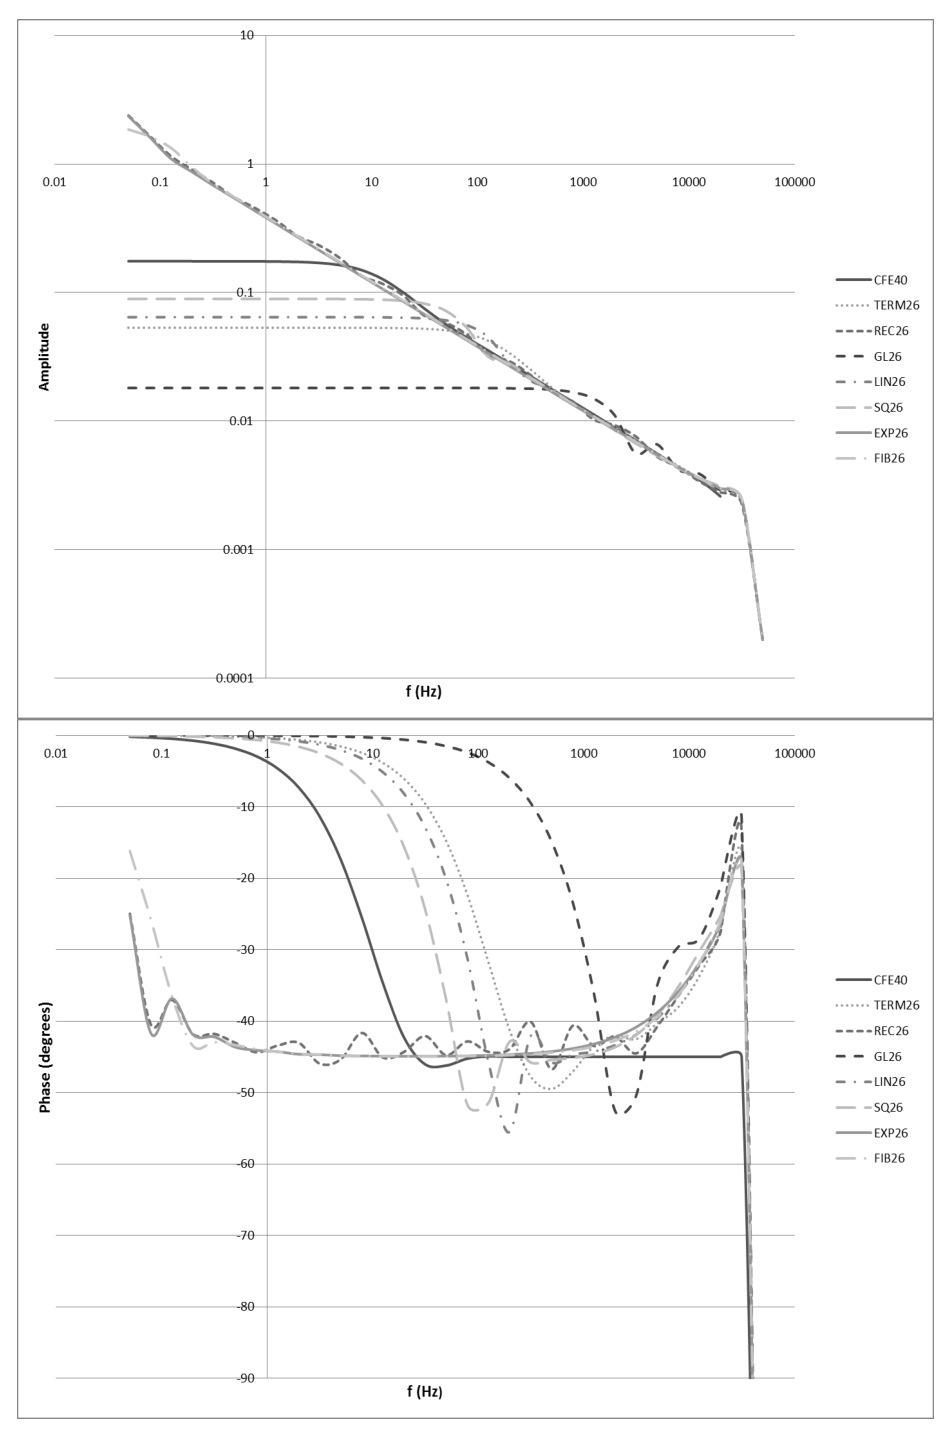
\includegraphics[width=2.5in]{bode1G_40_26_m05.eps}
}
\end{center}
\label{fig:bode40_26}
\caption{Bode plots for CFE with $40$ input signal history registers
  and average Grunwald with $26$ input signal history
  bins for $\alpha=0.5, 0.3, -0.3,$, and $-0.5$. }

\end{figure}
